%!TEX root = ../crimson_throne_book_main.tex
% 2015-10-10
\hyperref[fig:Chess-puzzle-in-the-Vivified-Labyrinth-565298239]{ The floor of the next room is paved with brown and white marble tiles, forming a big chessboard. Four queens line each side of the chamber. } A voice rings out as the heroes enter the room: "Eight queens are about to tear the realm apart. Only when they don't threaten each other there will be peace." At the same time a ticking starts, counting down the time the companions have to rearrange the pieces on the board. Pulling and pushing the heavy statues around, the young men succeed in getting six queens to a safe position, but when the timer stops after eight minutes, the two chess pieces that still threaten each other, animate and attack. It takes a lot of hits and healing before both marble figures are reduced to rubble on the floor. Combat continues in the room that follows. \hyperref[fig:Calikang-Vivified-Labyrinth-565300031]{ A calikang, a large blue-skinned, six-armed giant awakes from suspended animation and lurches to life, whirling around two sharp longswords and four clenched fists. } Puk gets the worst of it and needs to fall back on his halfling's luck ( he uses a hero point \\

\begin{figure}[h]
	\centering
	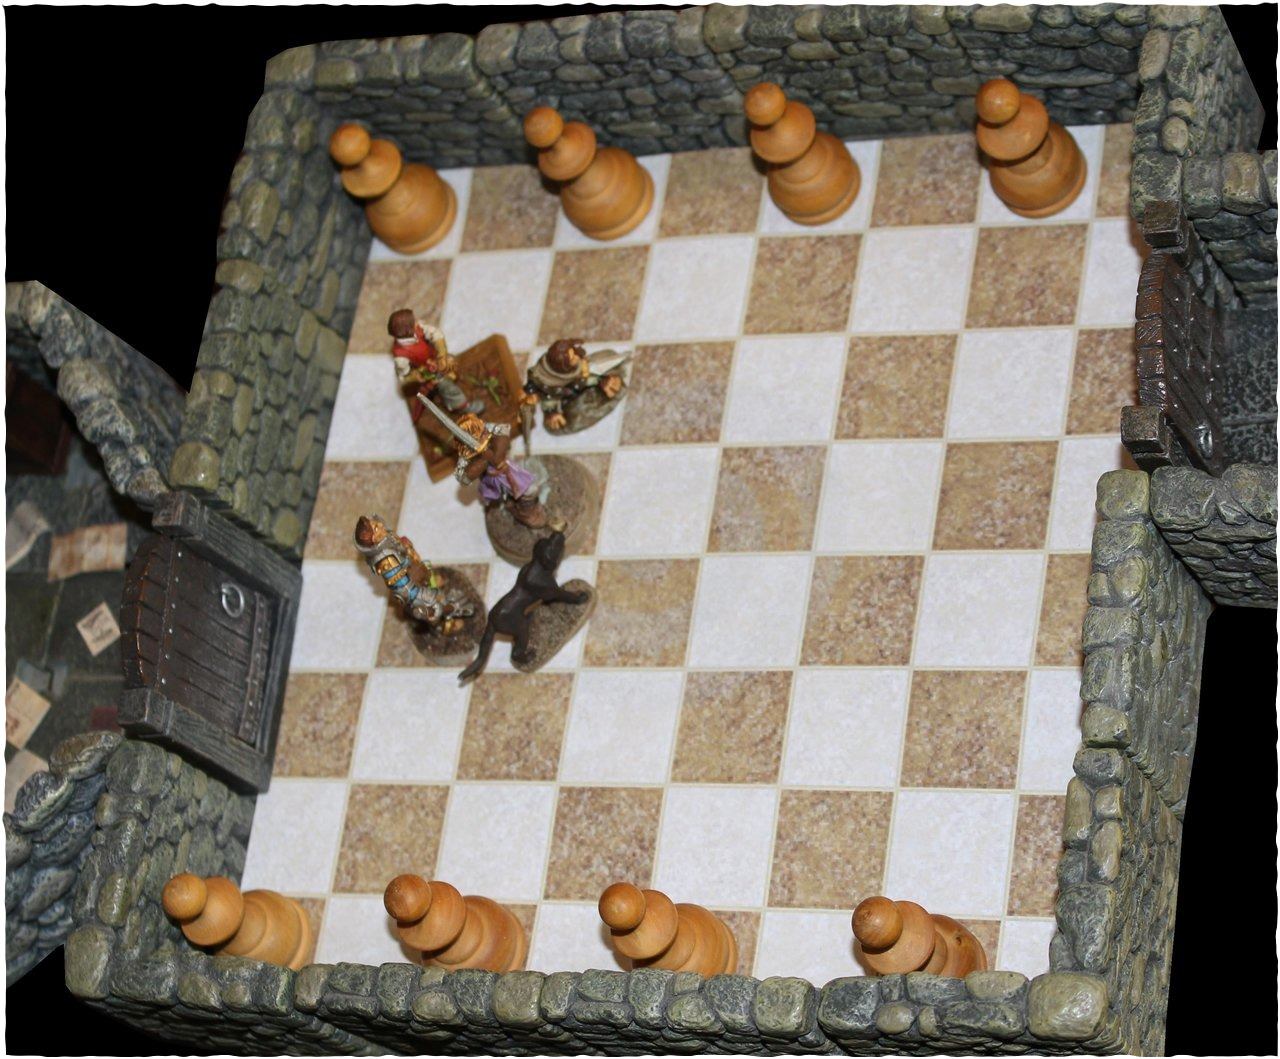
\includegraphics[width=0.4\textwidth]{images/Chess-puzzle-in-the-Vivified-Labyrinth-565298239_mod.jpg}
	\caption{Chess puzzle in the Vivified Labyrinth}
	\label{fig:Chess-puzzle-in-the-Vivified-Labyrinth-565298239}
\end{figure}

\begin{figure}[h]
	\centering
	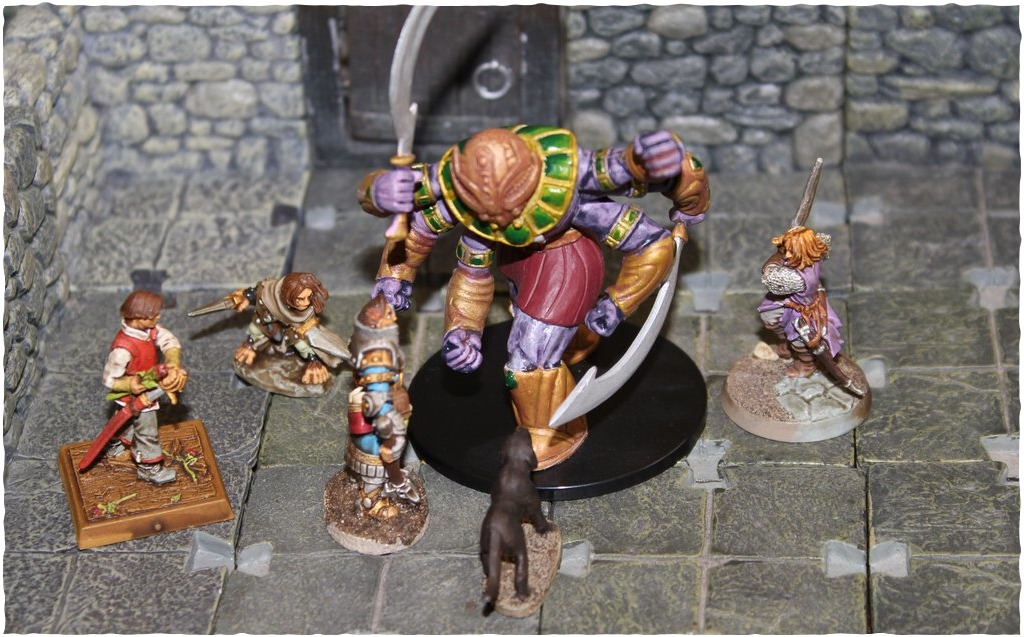
\includegraphics[width=0.4\textwidth]{images/Calikang-Vivified-Labyrinth-565300031_mod.jpg}
	\caption{Calikang Vivified Labyrinth}
	\label{fig:Calikang-Vivified-Labyrinth-565300031}
\end{figure}

The next puzzle takes place in a vaguely-heart-shaped room with two magic circles on the floor: one glowing in red and the other radiating blue light.\hyperref[fig:Fire-and-water-in-the-Vivified-Labyrinth-565300388]{ The companions are teleported to a square in the middle, as two elemental appear in front of the way in and the way out. } Behind them the heroes see a large water elemental, who speaks to them in a low voice: "My name is Rivers, I will follow." In front of them is a fire elemental who bellows: "My name is Pyro, I will oppose!" While the water elemental mimics the companions' movements, the fire elemental does the exact opposite. Using the walls and corners to get one or both elementals to stay in place as they move themselves, our friends manage to lure Rivers to the blue circle and Pyro to the red one. The elementals fall into a passive state as the final door clicks open. \\

\begin{figure}[h]
	\centering
	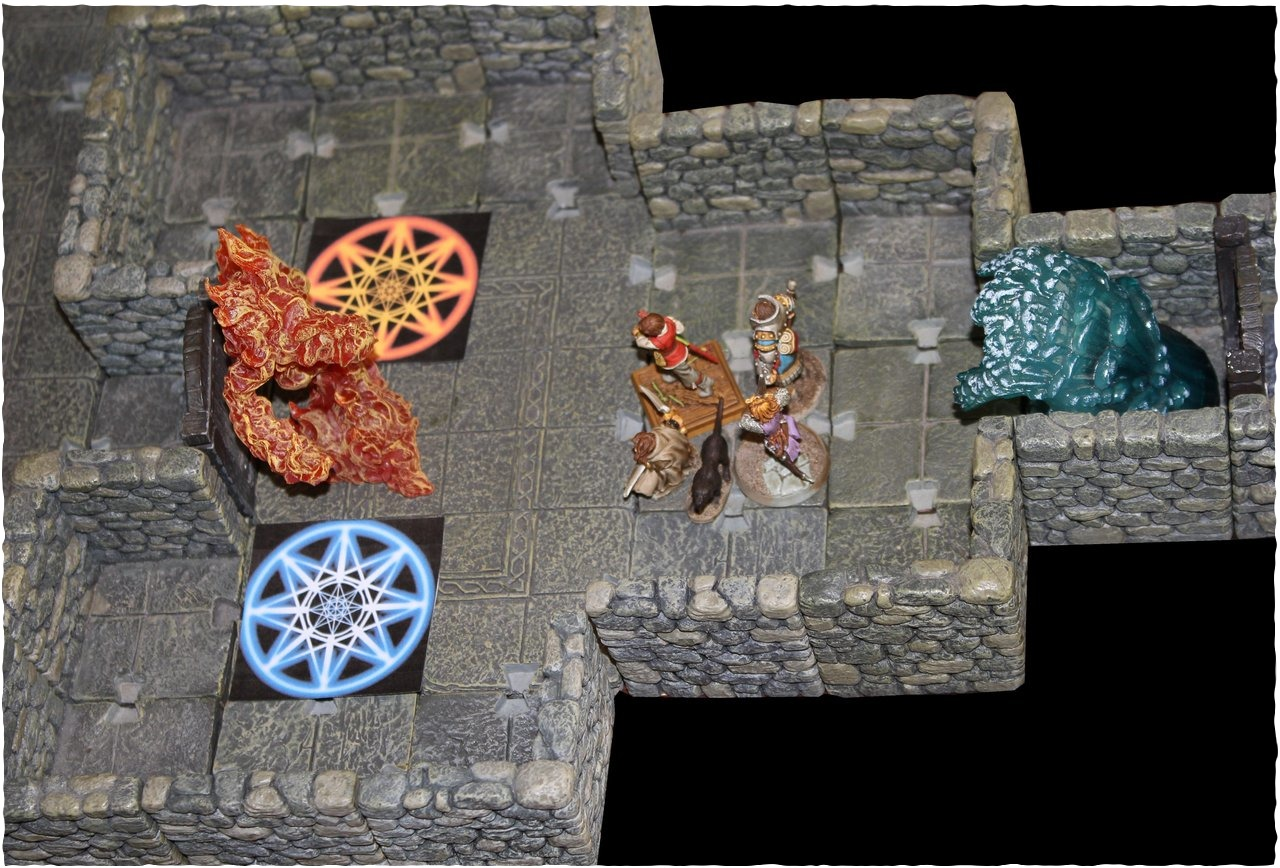
\includegraphics[width=0.4\textwidth]{images/Fire-and-water-in-the-Vivified-Labyrinth-565300388_mod.jpg}
	\caption{Fire and water in the Vivified Labyrinth}
	\label{fig:Fire-and-water-in-the-Vivified-Labyrinth-565300388}
\end{figure}

\hyperref[fig:Vivified-labyrinth25-565301156]{ The final chamber of the labyrinth is richly decorated with a luxurious bed, an impressive throne } and beautiful frescoes covering the walls. There are three vats against the wall across the entrance, providing porridge, water and wine. When the companions enter, a woman, bearing a close resemblance to the divine statue of Chamidu in the Arkona palace, approaches. \hyperref[fig:Nerio-Arkona-s-treasure-565301563]{ She carries three exotic weapons in her six hands, a curved longsword, a kukri and a long spear. } Her head holds three golden-skinned faces, which are paragons of physical perfection except for the large curved fangs curling out of their mouths. Her ears are pointed like an elf's, and like the slender fair creature, she moves with grace in her flowing azure dress. Still, her intentions do not seem so lovely as she greets her visitors: "So, after all these decades my descendants finally send in their minions again ... Don't they realize that you are only here to become my playthings? So, little dolls, let's play ..." Next she initiates combat. \\

\begin{figure}[h]
	\centering
	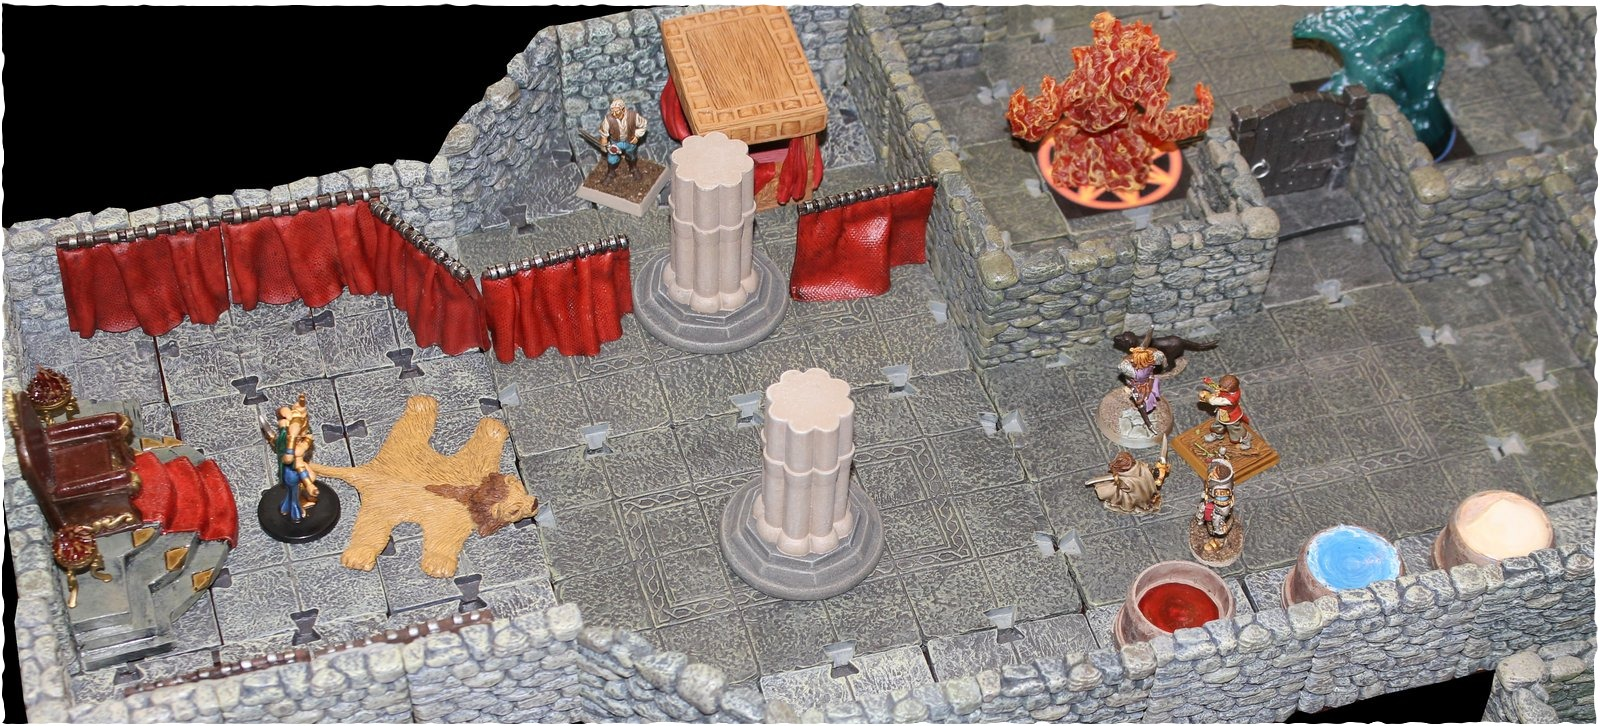
\includegraphics[width=0.4\textwidth]{images/Vivified-labyrinth25-565301156_mod.jpg}
	\caption{Vivified labyrinth25}
	\label{fig:Vivified-labyrinth25-565301156}
\end{figure}

\begin{figure}[h]
	\centering
	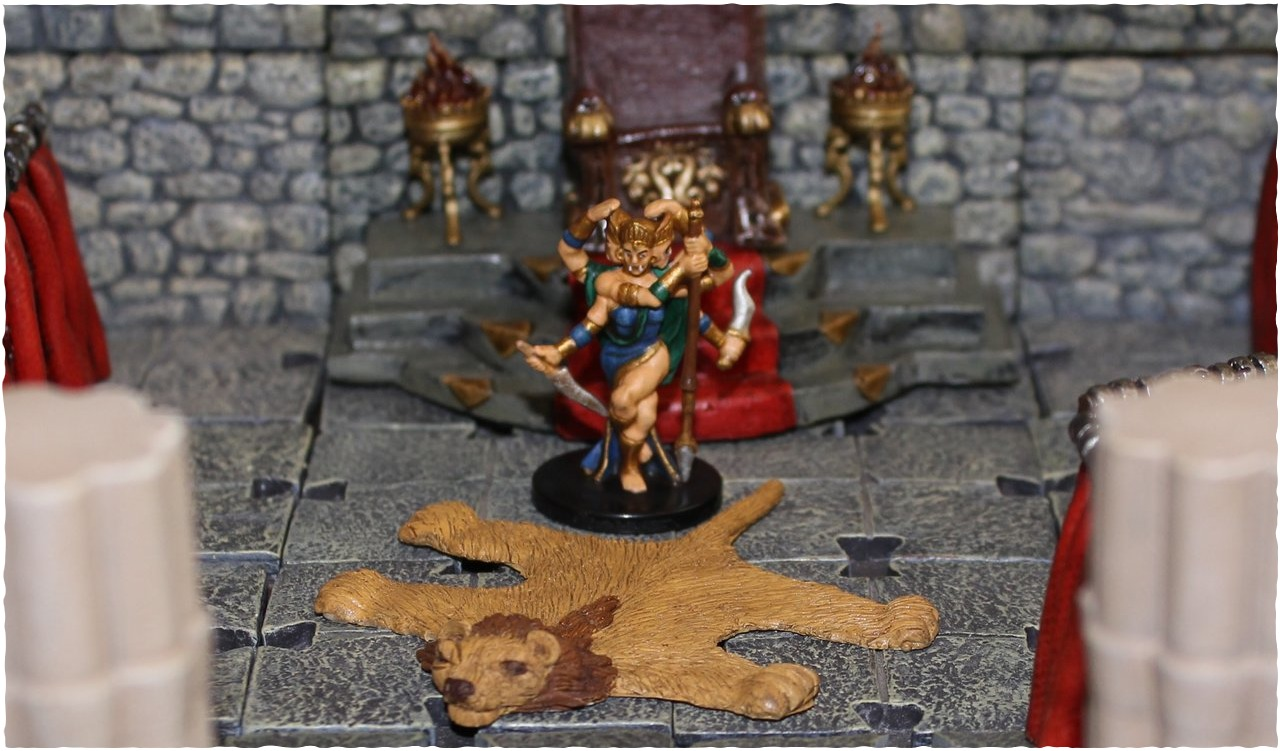
\includegraphics[width=0.4\textwidth]{images/Nerio-Arkona-s-treasure-565301563_mod.jpg}
	\caption{Nerio Arkona's treasure}
	\label{fig:Nerio-Arkona-s-treasure-565301563}
\end{figure}

Quint starts mocking the creature, reducing her fighting prowess somewhat with his {\itshape satire} . But the many-armed woman has multiple attacks and starts toying with her assailants nonetheless, by lashing out at each of them. Balian, Puk and Spyder try to damage her with their attacks, but find it hard to get through her  {\itshape damage reduction} , while Sjo and Quint discover that magic has even less chance of affecting her. The two fall back on their healing, Sjo with his spells and Quint with his  {\itshape wand of cure serious wounds} to keep their friends in the fight. They also notice that the 'upasundra' has a innate power that heals her wounds while she fights. After having dealt some damage left and right, the six-armed warrioress suddenly changes tactics and starts focus-firing her enemies. Her many attacks take out Balian first. Sjo reaches for his newly discovered scroll of  {\itshape heal} and brings the ranger back to full health as Puk becomes the next victim of the upasundra's focus fire. Quint does his best to keep the halfling on his feet, but cannot keep up with the many wounds he is being dealt. Balian survives another burst of pummels and cuts and hacks mercilessly at the Vudran fighting machine. Quint restores Puk to consciousness, but the halfling is hit down again. After a truly brutal fight the heroes win out and finish the upasundra off. The chamber holds some extra revelations. The upasundra's crown turns out to be a {\itshape headband of charisma +4} . Vencarlo Orisini is lying on the bed, unconscious. But the biggest surprise comes from the paintings on the walls. They tell the amazing history of the Arkona family. The first frescoes show how an impoverished nobleman sets out on a desperate quest aboard a ship named the  {\itshape Reprieve} . After facing storms, monsters, pirates, hunger and illness the survivors set foot on Vudran shore and sell the natives the 'exotic' goods of the northern lands. The nobleman, clearly Glorio's ancestor Nerio, gains great respect and wealth and manages to convince the maharaja to let him face a legendary six-armed and three-faced warrior princess in combat. He defeats and enslaves her, taking her home when he sails for Korvosa again. There he has the Vudran palace constructed and fathers a son with the upasundra. The child inherits more from his mother than her golden skin, though, he has a second face on the back of his head. The pictures of him as a grown man show him with the same (front) face as Nerio's son Eduardo, but here his head is not covered with a shawl as on the painting in Glorio's lounge, revealing the creepy second face on the other side of his head. One particularly remarkable fresco has Eduardo standing over Nerio's dead body. The young nobleman clutches his head between his hands while both faces are screaming madly. From the shadows the upasundra watches. The final works portray the construction of the \hyperref[fig:Overview-of-the-Vivified-labyrinth-565302683]{ Vivified Labyrinth } , Nerio sending his 'mother' inside and enchanting the entrance to lock her in. \\

\begin{figure}[h]
	\centering
	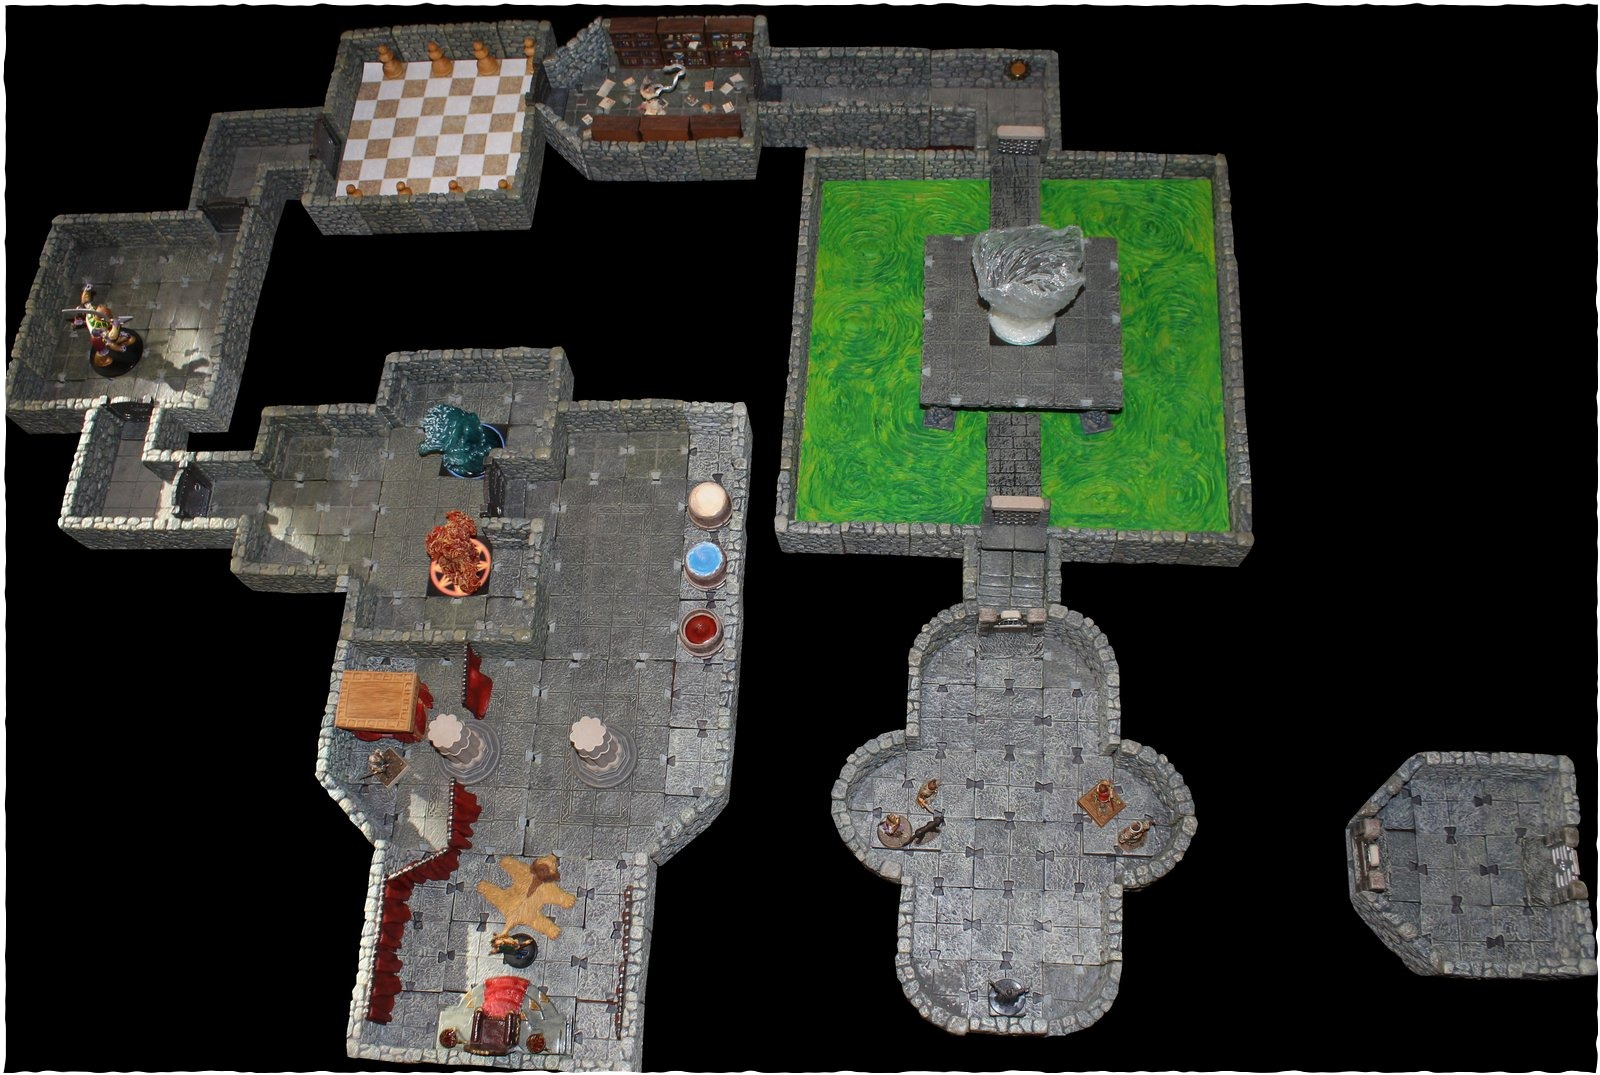
\includegraphics[width=0.4\textwidth]{images/Overview-of-the-Vivified-labyrinth-565302683_mod.jpg}
	\caption{Overview of the Vivified labyrinth}
	\label{fig:Overview-of-the-Vivified-labyrinth-565302683}
\end{figure}

So, Nerio's treasure was a creature that turns out to be Glorio's ancestor. The companions wonder if even the man himself knows ...\\

